% !TEX root = Projektdokumentation.tex
\begin{titlepage}

\begin{center}
\includegraphics[scale=0.2]{\IHKlogo}\\[0.5ex]
\Large{\ausbildungsberuf}\\
\LARGE{\betreff}\\
\huge{\textbf{\titelOne\\\titelTwo}}\\[0.5ex]
\Large{\textbf{\untertitelOne}}\\
\Large{\textbf{\untertitelTwo}}\\[1.5ex]

\normalsize
\textbf{Auszubildender:} \autorName\\[2.5ex]

\begin{figure}[htb]
    \centering
    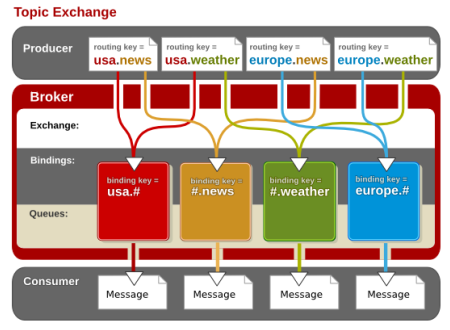
\includegraphics[scale=0.85]{\amqp}\\[1ex]
    \caption{Interprozesskommunikation mit Messaging-Queues}
    \label{fig:redHatCom}
\end{figure}

\textbf{Abgabetermin:} \abgabeOrt{}, den \abgabeTermin\\[3ex]

\includegraphics[scale=0.45]{\betriebLogo}\\
\betriebName{}\\
\betriebAnschrift{}, \betriebOrt\\[2.5ex]
\end{center}

\small
\noindent
Dieses Werk einschließlich seiner Teile ist \textbf{urheberrechtlich geschützt}.
Jede Verwertung außerhalb der engen Grenzen des Urheberrechtsgesetzes ist ohne Zustimmung des Autors unzulässig und strafbar.
Das gilt insbesondere für Vervielfältigungen, Übersetzungen, Mikroverfilmungen sowie die Einspeicherung und Verarbeitung in elektronischen Systemen.

\end{titlepage}